\section{Tests}

\begin{sectionbox}
	\subsection{Neyman-Pearson-Test}
	The best test of $\P_0$ against $\P_1$ is\\
	\parbox{15em}{$d_{\ir NP}(x) = \begin{cases} 1 & R(x) > c\\ γ & R(x) = c \\ 0 & R(x) < c \end{cases}$} \quad \parbox{15em}{ Likelihood-Ratio: \\ $R(x) = \frac{f_{\X}(x; θ_1)}{f_{\X}(x; θ_0)}$ }\\
	$γ = \frac{α - \P_0(\{R > c\})}{\P_0(\{R = c\})}$ \quad Errorlevel $α$\\
	Steps: For $α$ calculate $x_{α}$, then $c = R(x_{α})$\\
	\\
	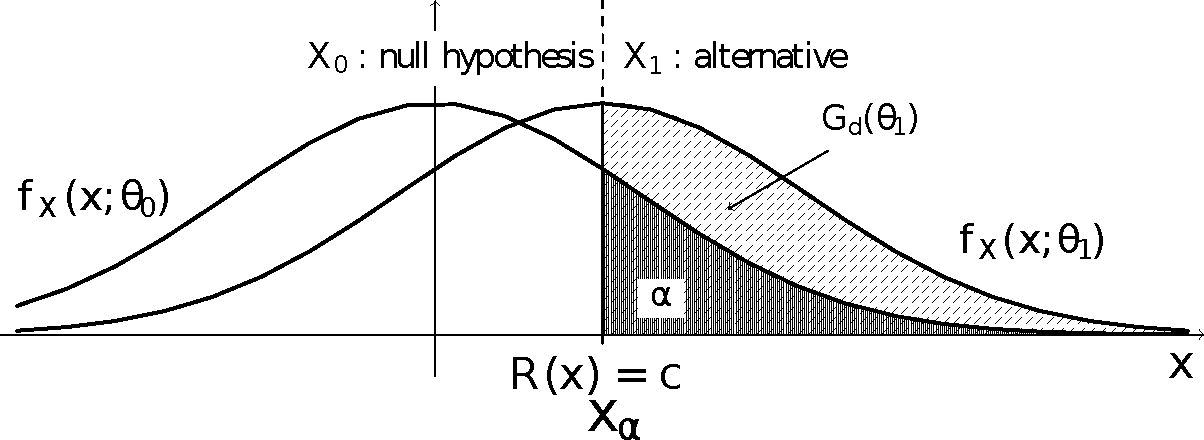
\includegraphics[width = 0.9\columnwidth]{tests}

	\textbf{Maximum Likelihood Detector:} \quad
	$d_{\ir ML}(x) = \begin{cases} 1 & R(x) > 1 \\ 0 & \text{otherwise} \end{cases}$\\
	\textbf{ROC Graphs:} plot $G_d(θ_1)$ as a function of $G_d(θ_0)$
\end{sectionbox}


\begin{sectionbox}
	\subsection{Bayes Test (MAP Detector)}
	Prior knowledge on possible hypotheses: $\P(\{θ ∈ Θ_0 \}) + \P(\{θ ∈ Θ_1\}) = 1$, minimizes the probability of a wrong
decision.\\
	$d_{\ir Bayes} =\! \begin{cases} 1& \!\frac{f_{\X}(x|θ_1)}{f_{\X}(x|θ_0)} > \frac{c_0 \P(θ_0|x)}{c_1 \P(θ_1|x)}\\ 0 & \text{otherwise} \end{cases}$
	$=\! \begin{cases} 1&\!\! \P(θ_1|x) > \P(θ_0|x) \\ 0 &\!\! \text{otherwise} \end{cases}$
	Risk weights $c_0,c_1$ are 1 by default.\\
	If $\P(θ_0) = \P(θ_1)$, the Bayes test is equivalent to the ML test\\
	\textbf{Loss Function} $L(d(x), θ) = \begin{cases} c_0 & \text{type 1 } d(x) = 1, \text{ but }θ = θ_0 \\ c_1 & \text{type 2 } d(x) = 0, \text{ but }θ = θ_1 \end{cases}$
	$\operatorname{risk}(d) = \E[L(d(\X), θ)] = \E [\E [L(d(x), θ)|x = \X ]]$\\
	\textbf{Multiple Hypothesis}
	$d_{\ir Bayes} = \begin{cases} 0 & x ∈ \mathbb X_0 \\ 1 & x ∈ \mathbb X_1 \\ 2 & x ∈ \mathbb X_2 \end{cases}$
\end{sectionbox}


\begin{sectionbox}
	\subsection{Linear Alternative Tests}
	$d: \mathbb X \ra \R, \vec x \mapsto \begin{cases} 1 & \vec w^\top \vec x - w_0 > 0 \\ 0 & \text{otherwise}\end{cases}$\\
	Estimate normal vector $\vec w^\top$, which separates $\mathbb X$ into $\mathbb X_0$ and $\mathbb X_1$\\
	$\log R(\vec x) = \frac{\ln(\det(\ma C_0))}{\ln(\det(\ma C_1))} + \frac{1}{2}(\vec x- \vec{μ}_0)^\top\ma C_0^{-1}(\vec x- \vec{μ}_0) -$ \\ $-\frac{1}{2}(\vec x- \vec{μ}_1)^\top\ma C_1^{-1}(\vec x- \vec{μ}_1) = 0$\\
	\textbf{For 2 Gaussians}, with $\ma C_0 = \ma C_1= \ma C$: $\vec w^\top = (\vec {μ}_1 - \vec{μ}_0)^\top \ma C$\\
	and constant translation $w_0 = \frac{(\vec {μ}_1 - \vec{μ}_0)^\top \ma C (\vec {μ}_1 - \vec{μ}_0)}{2}$\\


	% Bild aus Part7 p 197!!!
	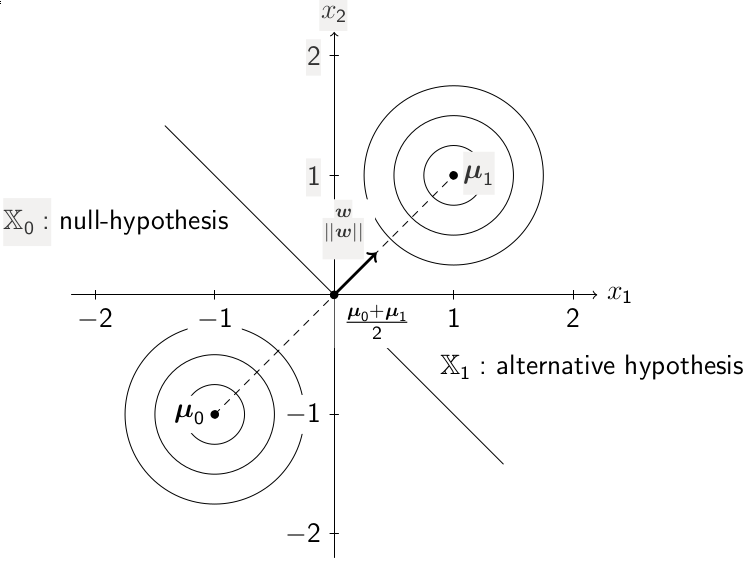
\includegraphics[width = 0.9\columnwidth]{linest2}
\end{sectionbox}
